\documentclass{article}
% For math environments
\usepackage{amsmath, amsfonts}
% For links
\usepackage[colorlinks=true,
    linkcolor = blue,
    urlcolor  = blue,
    citecolor = blue,
    anchorcolor = blue]{hyperref}
% Put space between paragraphs
\usepackage{parskip}
% For figures
\usepackage{tikz}
% Set the margins to not be ridiculous
\usepackage[margin=0.75in]{geometry}
% For multiple columns
\usepackage{multicol}
% For controlling enum/itemize spacing and indentation
\usepackage{enumitem}
% More math symbols
\usepackage{amssymb}
% To change enumerate labels

% For tikz plots
\usepackage{pgfplots}
% This isn't needed but avoids a compiler warning
\pgfplotsset{compat=1.16}

% Allow multi-line equations to be broken across pages
\allowdisplaybreaks

% Use @ as a letter
\makeatletter

% Scale down all tikz coordinates while maintaining font size
\tikzset{every picture/.style={scale=0.45, every picture/.style={}}}


% Macros
% Monospace code
\def\code#1{\texttt{#1}}

% Greek letters
\def\a{\alpha}
\def\b{\beta}
\def\g{\gamma}
\def\d{\delta}
\def\D{\Delta}

% Commands that make life easier
\newcommand\gath[1]{\begin{gather} #1 \end{gather}}
\newcommand\ali[1]{\begin{align} #1 \end{align}}
\newcommand\parens[1]{\left( #1 \right)}
\newcommand\squares[1]{\left[ #1 \right]}
\newcommand\braces[1]{\left\{ #1 \right\}}
\newcommand\angles[1]{\left\langle #1 \right\rangle}
\newcommand\deriv[2]{\frac{d #1}{d #2}}
\newcommand\abs[1]{\left| #1 \right|}
\newcommand\floor[1]{\left\lfloor #1 \right\rfloor}
\DeclareMathOperator{\lcm}{lcm}
\def\non{\nonumber \\}

% Multiline equation space
\def\mlesp{\hspace{1.2cm}}

% For grid diagrams
\newcommand\gridbox[3]{\draw (#1,#2) rectangle (#1+1,#2+1) node[pos=.5] {#3};}
\newcommand\gridboxh[3]{\draw[fill=red!20] (#1,#2) rectangle (#1+1,#2+1) node[pos=.5] {#3};}
\newcommand\gridboxb[3]{\draw[fill=black] (#1,#2) rectangle (#1+1,#2+1) node[pos=.5] {#3};}
\newcommand\gridsym[3]{\node at (#1+0.5,#2+0.5) {$#3$};}
\newcommand\gridblank[2]{\filldraw[draw=gray, color=gray] (#1,#2) rectangle (#1+1,#2+1);}
\newcommand\gridcirc[2]{\draw (#1 + 0.5,#2 + 0.5) circle (0.25);}
\newcommand\cwlab[3]{
  \def\dd{0.15}
  \draw (#1 + \dd - 0.03, #2 + 1 - \dd) node {\scriptsize #3};
}

\def\bbw{3.5}
\def\bbh{2}
\newcommand\bigbox[3]{\draw (#1*\bbw,#2*\bbh) rectangle (#1*\bbw+\bbw,#2*\bbh+\bbh) node[pos=.5] {#3};}
\newcommand\bbtextr[3]{\node[right] at (#1*\bbw,#2*\bbh+0.5*\bbh) {#3};}
\newcommand\bbtextb[3]{\node[align=center] at (#1*\bbw+0.5*\bbw,#2*\bbh+0.5*\bbh) {#3};}

% Box puzzle stock answer
\newcommand\boxans[1]{
  Logic was used to deduce the solution:

  #1

  This was verified using Python as well as shown to be unique with a brute force approach.
}

% Multiple numbers
\newcommand\mn[1]{$#1$'s}

% Commands for problems
\newcommand\problem[4]{
  \section*{#1}

  Question: #3
  
  Answer: #2
  
  Explanation: #4
}
\newcommand\aproblem[4]{\problem{Dec #1}{#2}{#3}{#4}}
\newcommand\cproblem[4]{\problem{Problem #1}{#2}{#3}{#4}}

\def\advent@xxiv@i{
  Eve writes down five different positive integers.
  The sum of her integers is $16$. What is the product of her integers?
}

\def\advent@xxiv@ii{
  $14$ is the smallest even number that cannot be obtained by rolling two $6$-sided dice and finding the product of the numbers rolled.

  What is the smallest even number that cannot be obtained by rolling one hundred $100$-sided dice and finding the product of the numbers rolled?
}

\def\advent@xxiv@iii{
  There are $5$ ways to write $5$ as the sum of positive odd numbers:
  \begin{itemize}
    \item $1 + 1 + 1 + 1 + 1$
    \item $1 + 1 + 3$
    \item $3 + 1 + 1$
    \item $1 + 3 + 1$
    \item $5$
  \end{itemize}

  How many ways are there to write $14$ as the sum of positive odd numbers?
}

\def\advent@xxiv@iv{
  The geometric mean of a set of $n$ numbers is computed by mulitplying all the numbers together, then taking the $n$th root.
  The factors of $9$ are $1$, $3$, and $9$.
  The geometric mean of these factors is
  \gath{
    \sqrt[3]{1 \times 3 \times 9} = \sqrt[3]{27} = 3
  }
  What is the smallest number where the geometric mean of its factors is $13$?
}

\def\advent@xxiv@v{
  The sum of $11$ consecutive integers is $2024$.
  What is the smallest of the $11$ integers?
}

\def\advent@xxiv@vi{Put the digits 1 to 9 (using each digit exactly once) in the boxes so that the sums are correct. The sums should be read left to right and top to bottom ignoring the usual order of operations. For example, 4+3×2 is 14, not 10. Today's number is the product of the numbers in the red boxes.
  The number $n$ has $55$ digits.
  All of its digits are $9$.
  What is the sum of the digits of $n^3$?
}

\def\advent@xxiv@vii{
  What is the obtuse angle in degrees between the minute and hour hands of a clock at 08:22?
}

\def\advent@xxiv@viii{
  It is possible to arrange $4$ points on a plane and draw non-intersecting lines between them to form $3$ non-overlapping triangles:

  \begin{center}
    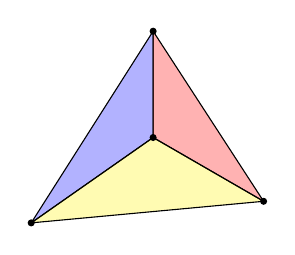
\begin{tikzpicture}
      \def\ds{3}
      \def\pa{(0: 0)}
      \def\pb{(90: \ds)}
      \def\pc{(215: 1.4*\ds)}
      \def\pd{(-30: 1.2*\ds)}

      \def\bcr{3}
      \def\scr{0.55*\bcr}
      \def\sca{34}
      \def\mcr{0.7*\bcr}
      \def\mca{142}
      \def\pr{0.1}

      % Triangles
      \draw[fill=blue,fill opacity=0.3] \pa -- \pb -- \pc -- cycle;
      \draw[fill=red,fill opacity=0.3] \pa -- \pb -- \pd -- cycle;
      \draw[fill=yellow,fill opacity=0.3] \pa -- \pd -- \pc -- cycle;

      % Points
      \fill \pa circle (\pr);
      \fill \pb circle (\pr);
      \fill \pc circle (\pr);
      \fill \pd circle (\pr);
    \end{tikzpicture}
  \end{center}

  It is not possible to make more than $3$ triangles with $4$ points.

  What is the maximum number of non-overlapping triangles that can be made by arranging $290$ points on a plane and drawing non-intersecting lines between them?
}

\def\advent@xxiv@ix{
  Put the digits $1$ to $9$ (using each digit exactly once) in the boxes so that the sums are correct.
  The sums should be read left to right and top to bottom ignoring the usual order of operations.
  For example, $4 + 3 \times 2$ is $14$, not $10$.
  Today's number is the product of the numbers in the red boxes.

  \grid@advent@xxiv@ix{}{}{}{}{}{}{}{}{}
}

\def\advent@xxiv@x{
  A number is a palindrome if it's the same when its digits are written in reverse order.

  What is the sum of all the numbers between $10$ and $100$ that are palindromes?
}

\def\advent@xxiv@xi{
  There are $6$ sets of integers between $1$ and $5$ (inclusive) that contain an odd number of numbers whose median value is $3$:

  \begin{itemize}
    \item $\braces{3}$
    \item $\braces{1,3,4}$
    \item $\braces{2,3,4}$
    \item $\braces{1,3,5}$
    \item $\braces{2,3,5}$
    \item $\braces{1,2,3,4,5}$
  \end{itemize}

  How many sets of integers between $1$ and $11$ (inclusive) are there that contain an odd number of numbers whose median value is $5$?
}

\def\advent@xxiv@xii{
  Holly picks a three-digit number.
  She then makes a two-digit number by removing one of the digits.
  The sum of her two numbers is $309$.
  What was Holly's original three-digit number?
}

\def\advent@xxiv@xiii{
  Today's number is given in this crossnumber.
  No number in the completed grid starts with $0$.

  \begin{multicols}{2}
    \crossnumstd{}{}{}{}{}{}{}{}{}

    \vfill\null
    \columnbreak

    \begin{center}
      \textbf{Across}

      \begin{tabular}{clc}
        \textbf{1} & Today's number.  & (\textbf{3}) \\
        \textbf{4} & Two times 5A.    & (\textbf{3}) \\
        \textbf{5} & A multiple of 1. & (\textbf{3})
      \end{tabular}

      \textbf{Down}

      \begin{tabular}{clc}
        \textbf{1} & Sum of digits is 15. & (\textbf{3}) \\
        \textbf{2} & Sum of digits is 19. & (\textbf{3}) \\
        \textbf{3} & Three times 5A.      & (\textbf{3})
      \end{tabular}
    \end{center}
  \end{multicols}
}

\def\advent@xxiv@xiv{
  $15^3$ is $3375$.
  The last $3$ digits of $15^3$ are $375$.

  What are the last $3$ digits of $15^{1234567890}$?
}

\def\advent@xxiv@xv{
  The number $2268$ is equal to the product of a square number (whose last digit is not $0$) and the same square number with its digits reversed: $36 \times 63$.

  What is the smallest three-digit number that is equal to the product of a square number (whose last digit is not $0$) and the same square number with its digits reversed?
}

\def\advent@xxiv@xvi{
  Put the digits $1$ to $9$ (using each digit exactly once) in the boxes so that the sums are correct.
  The sums should be read left to right and top to bottom ignoring the usual order of operations.
  For example, $4 + 3 \times 2$ is $14$, not $10$.
  Today's number is the product of the numbers in the red boxes.

  \grid@advent@xxiv@xvi{}{}{}{}{}{}{}{}{}
}

\def\advent@xxiv@xvii{
  The number $40$ has $8$ factors: $1$, $2$, $4$, $5$, $8$, $10$, $20$, and $40$.

  How many factors does the number $2^{26} \times 5 \times 7^5 \times 11^2$ have?
}

\def\advent@xxiv@xviii{
  TODO
}

\def\card@xxiv@i{
  What is the largest number you can make by using the digits $1$ to $4$ to make two $2$-digit numbers, then mutiplying the two numbers together?
}

\def\card@xxiv@ii{
  What is the largest number you can make by using the digits $0$ to $9$ to make a $2$-digit number and an $8$-digit number, then mutiplying the two numbers together?
}

\def\card@xxiv@iii{
  The expansion of $(2x+3)^2$ is $4x^2 + 12x + 9$.
  The sum of the coefficients of $4x^2 + 12x + 9$ is $25$.
  What is the sum of the coefficients of the expansion of $(30x + 5)^2$?
}

\def\card@xxiv@iv{
  What is the sum of the coefficients of the expansion of $(2x+1)^{11}$?
}

\def\card@xxiv@v{
  What is the geometric mean of all the factors of $41306329$?
}

\def\card@xxiv@vi{
  What is the largest number for which the geometric mean of all its factors is $92$?
}

\def\card@xxiv@vii{
  What is the sum of all the factors of $7^4$?
}

\def\card@xxiv@viii{
  How many numbers between $1$ and $28988500000$ have an odd number of factors?
}

\def\card@xxiv@ix{
  Eve found the total of the $365$ consecutive integers starting at $500$ and the total of the next $365$ consecutive integers, then subtracted the smaller total from the larger total.
  What was her result?
}

\def\card@xxiv@x{
  Eve found the total of the $n$ consecutive integers starting at a number and the total of the next $n$ consecutive integers, then subtracted the smaller total from the larger total.
  Her result was $22344529$.
  What is the largest possible value of $n$ that she could have used?
}

\input{boxes}

\begin{document}

\title{MS Scroggs Advent Calendar 2022 Answers}
\author{Dan Whitman}
\date{}

\maketitle

% TODO: Once the event is over, add answers link.
%Answers: \href{https://www.mscroggs.co.uk/puzzles/advent2021}{https://www.mscroggs.co.uk/puzzles/advent2021}
Synchronized calendar: \href{http://mscroggs.co.uk/adventcode/JYcziCbI}{http://mscroggs.co.uk/adventcode/JYcziCbI}

\aproblem{1}{162}{\advent@xxii@i}{
  Since $p_1 = (9,0)$ is a vertex and the $y$-axis is a line of symmetry, it must be that a second vertex is $p_2 = (-9, 0)$.
  Since there must be four vertices, and both $p_1$ and $p_2$ are on the $x$-axis, it must be that the other two vertices are on the $y$-axis.
  This is because any vertex not on either axis would result in four vertices not on either axis due to the axes being lines of symmetry, and a rectangle cannot have six vertices!
  It then must be that the two $y$-axis vertices are at $p_3 = (0, 9)$ and $p_4 = (0, -9)$, since any other points that possess the required symmetry would result in a parallelogram without right angles.

  Therefore, our rectangle is also square that clearly has sides of $s = \sqrt{9^2 + 9^2} = 9\sqrt{2}$.
  The area is then of course $A = s^2 = 81 \cdot 2 = 162$.
}

\aproblem{2}{840}{\advent@xxii@ii}{
  Clearly $1$, $2$, $3$, $5$, and $7$ are prime whereas $4 = 2^2$, $6 = 2 \cdot 3$, and $8 = 2^3$.
  Therefore we have that
  \gath{
    \lcm(1, 2, 3, 4, 5, 6, 7, 8) = 2^3 \cdot 3 \cdot 5 \cdot 7 = 840 \,.
  }
}

\aproblem{3}{369}{\advent@xxii@iii}{
  Suppose that for the $n$th row we choose the element in the $p_n$th column (where $1 \leq n, p_n \leq 9$).
  Since we must only choose exactly one number in each column, clearly for any permutation we have that $\braces{p_n \mid 1 \leq n \leq 9} = \braces{1, 2, \ldots, 9}$, and hence
  \gath{
    \sum_{n=1}^9 p_n = 1 + 2 + \ldots + 9 = \sum_{i=1}^9 i = \frac{9 \cdot 10}{2} = 45 \,.
  }
  Now, if $x_n$ is the selected value of the $n$th row, then this value is reasoned to be
  \gath{
    x_n = 9(n-1) + p_n \,.
  }
  Hence, the sum of all the selected values is always
  \gath{
    \sum_{n=1}^9 x_n = \sum_{n=1}^9 \squares{9(n-1) + p_n} = 9 \sum_{n=1}^9 n - 9 \sum_{n=1}^9 1 + \sum_{n=1}^9 p_n
    = 9 \cdot 45 - 9 \cdot 9 + 45 = 369
  }
  regardless of the selection permutation.
  This result was verified by a brute force Python program.
}

\aproblem{4}{625}{\advent@xxii@iv}{
  First, clearly the last three digits of any number $n \geq 100$ is just $n \mod 1000$.
  We claim, for all $n \geq 3$, that
  \gath{
    5^n \mod 1000 = \begin{cases}
      625 & \text{$n$ is even}    \\
      125 & \text{$n$ is odd} \,,
    \end{cases}
  }
  which we show by induction on $n$.
  First, for $n = 3$, we obviously have $5^3 = 125 \equiv 125 \pmod{1000}$ so that the hypothesis is true here since $n = 3$ is odd.
  Now suppose that the hypothesis is true for $n$.
  If $n$ is even then $5^n \equiv 625 \pmod{1000}$ so that
  \gath{
    5^{n+1} = 5 \cdot 5^n \equiv 5 \cdot 625 \pmod{1000} \equiv 3125 \pmod{1000} \equiv 125 \pmod{1000},
  }
  which proves the hypothesis for $n+1$ since $n+1$ is odd.
  If, on the other hand, $n$ is odd, then $5^n \equiv 125 \pmod{1000}$ by the induction hypothesis so that
  \gath{
    5^{n+1} = 5 \cdot 5^n \equiv 5 \cdot 125 \pmod{1000} \equiv 625 \pmod{1000},
  }
  which again proves the hypothesis for $n+1$ since here $n+1$ is even.

  Now, since clearly $n = 2022000000$ is even, it follows that the last three digits of $5^n$ are $625$ by what was just proven.
}

\aproblem{5}{315}{\advent@xxii@v}{
  \boxans{\gridsol@advent@xxii@v}
}

\aproblem{6}{128}{\advent@xxii@vi}{
  First, consider a general sum digit $1 \leq s \leq 9$, and let $N_m(s)$ denote the number of $m$-digit numbers such that the digits are all non-zero digits and add to $s$.
  Clearly $N_1(s) = 1$, namely the single digit $s$ itself.
  Next, consider $m$-digit numbers for $m > 1$.
  If the first digit is $1$, then there are $N_{m-1}(s-1)$ combinations of remaining digits so that to overall digital sum is $s$.
  Likewise, if the first digit is $2$, then there are $N_{m-1}(s-2)$ combinations of remaining digits.

  More generally, if the first digit is $1 \leq i \leq s - (m-1)$, then there are $N_{m-1}(s - i)$ combinations of remaining digits such that the overall digital sum is $s$.
  Note that $i \leq s - (m-1)$ since the minimal sum of the remaining digits is $m-1$, namely when they are all \mn{1}.
  Therefore, considering all the first digits, we have the recursive equation
  \gath{
    N_m(s) = \sum_{i=1}^{s - (m-1)} N_{m-1}(s - i) = \sum_{j=m-1}^{s-1} N_{m-1}(j), \label{eqn:06:rec}
  }
  where we have changed indices using $j = s - i$.
  Also note that it must be that $m \leq s$ since there are no terms otherwise, and $m = s$ corresponds to an $s$-digit number with a digital sum $s$ so that all digits must be \mn{1}, and hence $N_s(s) = 1$.

  For a given $s$, it follows that the total number of qualifying integers (with any number of digits) with that digital sum is then
  \gath{
    N_s = \sum_{m=1}^s N_m(s). \label{eqn:06:main}
  }
  Now, we have
  \gath{
    N_2(s) = \sum_{j=1}^{s-1} N_1(j) = \sum_{j=1}^{s-1} 1 = (s - 1) - 1 + 1 = s - 1
  }
  and
  \ali{
    N_3(s) &= \sum_{j=2}^{s-1} N_2(j) = \sum_{j=2}^{s-1} (s - 1) = \sum_{j=2}^{s-1} s - \sum_{j=2}^{s-1} 1 = \squares{\frac{s(s-1)}{2} - 1} - (s - 2) \non
    &= \frac{s(s-1)}{2} - s + 1 = \frac{s(s-1) - 2s + 2}{2} = \frac{s^2 - 3s + 2}{2} = \frac{(s-1)(s-2)}{2}.
  }
  This could be continued to $N_4(s)$, $N_5(s)$, etc., but this would quickly become very tedious.
  In our case we are looking for $N_8$, for which we would need to determine $N_m(s)$ up through $N_8(s)$.
  Rather than endure this tedium, we simply implement the recursive function \eqref{eqn:06:rec} with the base case of $N_1(s) = 1$ in Python and use \eqref{eqn:06:main} to calculate $N_8 = 128$.

  This result was also verified with a brute force search in the Python program.
}

\aproblem{7}{476}{\advent@xxii@vii}{
  It seems fairly clear that the largest triangle that can fit within a hexagon is that whose three vertices lie on every other vertex of the hexagon as shown below:
  \def\hexr{3}
  \begin{center}
    \begin{tikzpicture}
      \draw (-30:\hexr) -- (30:\hexr) -- (90:\hexr) -- (150:\hexr) -- (210:\hexr) -- (270:\hexr) -- cycle;
      \draw[fill=red] (-30:\hexr) -- (90:\hexr) -- (210:\hexr) -- cycle;
    \end{tikzpicture}
  \end{center}
  Let $s$ denote the side length of the hexagon, and let $t$ denote the side of the inner red triangle, which is clearly equilateral.
  The three smaller white triangles inside the hexagon but outside the red triangle are isosceles and have two side of length $s$ and a base of length $t$.
  Moreover, the apex angles of these triangles is $120^\circ$, from which it follows that
  \gath{
    t = \sqrt{3} s
  }
  so that the area of the large red triangle is
  \gath{
    A_t = \frac{\sqrt{3}}{4} t^2 = \frac{\sqrt{3}}{4} \parens{\sqrt{3} s}^2 = \frac{3\sqrt{3}}{4} s^2.
  }
  Meanwhile, the area of the hexagon is
  \gath{
    A_h = \frac{3\sqrt{3}}{2} s^2.
  }
  Therefore, we have
  \gath{
    A_t = \frac{1}{2} A_h = \frac{1}{2} \cdot 952 = 476.
  }
}

\aproblem{8}{TODO}{\advent@xxii@viii}{
  TODO
}

\aproblem{9}{TODO}{\advent@xxii@ix}{
  TODO
}

\aproblem{10}{TODO}{\advent@xxii@x}{
  TODO
}

\aproblem{11}{TODO}{\advent@xxii@xi}{
  TODO
}

\aproblem{12}{TODO}{\advent@xxii@xii}{
  TODO
}

\aproblem{13}{TODO}{\advent@xxii@xiii}{
  TODO
}

\aproblem{14}{TODO}{\advent@xxii@xiv}{
  TODO
}

\aproblem{15}{TODO}{\advent@xxii@xv}{
  TODO
}

\aproblem{16}{TODO}{\advent@xxii@xvi}{
  TODO
}

\aproblem{17}{TODO}{\advent@xxii@xvii}{
  TODO
}

\aproblem{18}{TODO}{\advent@xxii@xviii}{
  TODO
}

\aproblem{19}{TODO}{\advent@xxii@xix}{
  TODO
}

\aproblem{20}{TODO}{\advent@xxii@xx}{
  TODO
}

\aproblem{21}{TODO}{\advent@xxii@xxi}{
  TODO
}

\aproblem{22}{TODO}{\advent@xxii@xxii}{
  TODO
}

\aproblem{23}{TODO}{\advent@xxii@xxiii}{
  TODO
}

\aproblem{24}{TODO}{\advent@xxii@xxiv}{
  TODO
}

\end{document}
